% Options for packages loaded elsewhere
% Options for packages loaded elsewhere
\PassOptionsToPackage{unicode}{hyperref}
\PassOptionsToPackage{hyphens}{url}
\PassOptionsToPackage{dvipsnames,svgnames,x11names}{xcolor}
%
\documentclass[
  spanish,
  a4paper,
  oneside]{scrbook}
\usepackage{xcolor}
\usepackage[top=25mm,bottom=25mm,left=30mm,right=20mm]{geometry}
\usepackage{amsmath,amssymb}
\setcounter{secnumdepth}{5}
\usepackage{iftex}
\ifPDFTeX
  \usepackage[T1]{fontenc}
  \usepackage[utf8]{inputenc}
  \usepackage{textcomp} % provide euro and other symbols
\else % if luatex or xetex
  \usepackage{unicode-math} % this also loads fontspec
  \defaultfontfeatures{Scale=MatchLowercase}
  \defaultfontfeatures[\rmfamily]{Ligatures=TeX,Scale=1}
\fi
\usepackage{lmodern}
\ifPDFTeX\else
  % xetex/luatex font selection
  \setmainfont[]{TeX Gyre Termes}
  \setsansfont[]{TeX Gyre Heros}
  \setmonofont[]{TeX Gyre Cursor}
\fi
% Use upquote if available, for straight quotes in verbatim environments
\IfFileExists{upquote.sty}{\usepackage{upquote}}{}
\IfFileExists{microtype.sty}{% use microtype if available
  \usepackage[]{microtype}
  \UseMicrotypeSet[protrusion]{basicmath} % disable protrusion for tt fonts
}{}
\makeatletter
\@ifundefined{KOMAClassName}{% if non-KOMA class
  \IfFileExists{parskip.sty}{%
    \usepackage{parskip}
  }{% else
    \setlength{\parindent}{0pt}
    \setlength{\parskip}{6pt plus 2pt minus 1pt}}
}{% if KOMA class
  \KOMAoptions{parskip=half}}
\makeatother
% Make \paragraph and \subparagraph free-standing
\makeatletter
\ifx\paragraph\undefined\else
  \let\oldparagraph\paragraph
  \renewcommand{\paragraph}{
    \@ifstar
      \xxxParagraphStar
      \xxxParagraphNoStar
  }
  \newcommand{\xxxParagraphStar}[1]{\oldparagraph*{#1}\mbox{}}
  \newcommand{\xxxParagraphNoStar}[1]{\oldparagraph{#1}\mbox{}}
\fi
\ifx\subparagraph\undefined\else
  \let\oldsubparagraph\subparagraph
  \renewcommand{\subparagraph}{
    \@ifstar
      \xxxSubParagraphStar
      \xxxSubParagraphNoStar
  }
  \newcommand{\xxxSubParagraphStar}[1]{\oldsubparagraph*{#1}\mbox{}}
  \newcommand{\xxxSubParagraphNoStar}[1]{\oldsubparagraph{#1}\mbox{}}
\fi
\makeatother

\usepackage{color}
\usepackage{fancyvrb}
\newcommand{\VerbBar}{|}
\newcommand{\VERB}{\Verb[commandchars=\\\{\}]}
\DefineVerbatimEnvironment{Highlighting}{Verbatim}{commandchars=\\\{\}}
% Add ',fontsize=\small' for more characters per line
\usepackage{framed}
\definecolor{shadecolor}{RGB}{241,243,245}
\newenvironment{Shaded}{\begin{snugshade}}{\end{snugshade}}
\newcommand{\AlertTok}[1]{\textcolor[rgb]{0.68,0.00,0.00}{#1}}
\newcommand{\AnnotationTok}[1]{\textcolor[rgb]{0.37,0.37,0.37}{#1}}
\newcommand{\AttributeTok}[1]{\textcolor[rgb]{0.40,0.45,0.13}{#1}}
\newcommand{\BaseNTok}[1]{\textcolor[rgb]{0.68,0.00,0.00}{#1}}
\newcommand{\BuiltInTok}[1]{\textcolor[rgb]{0.00,0.23,0.31}{#1}}
\newcommand{\CharTok}[1]{\textcolor[rgb]{0.13,0.47,0.30}{#1}}
\newcommand{\CommentTok}[1]{\textcolor[rgb]{0.37,0.37,0.37}{#1}}
\newcommand{\CommentVarTok}[1]{\textcolor[rgb]{0.37,0.37,0.37}{\textit{#1}}}
\newcommand{\ConstantTok}[1]{\textcolor[rgb]{0.56,0.35,0.01}{#1}}
\newcommand{\ControlFlowTok}[1]{\textcolor[rgb]{0.00,0.23,0.31}{\textbf{#1}}}
\newcommand{\DataTypeTok}[1]{\textcolor[rgb]{0.68,0.00,0.00}{#1}}
\newcommand{\DecValTok}[1]{\textcolor[rgb]{0.68,0.00,0.00}{#1}}
\newcommand{\DocumentationTok}[1]{\textcolor[rgb]{0.37,0.37,0.37}{\textit{#1}}}
\newcommand{\ErrorTok}[1]{\textcolor[rgb]{0.68,0.00,0.00}{#1}}
\newcommand{\ExtensionTok}[1]{\textcolor[rgb]{0.00,0.23,0.31}{#1}}
\newcommand{\FloatTok}[1]{\textcolor[rgb]{0.68,0.00,0.00}{#1}}
\newcommand{\FunctionTok}[1]{\textcolor[rgb]{0.28,0.35,0.67}{#1}}
\newcommand{\ImportTok}[1]{\textcolor[rgb]{0.00,0.46,0.62}{#1}}
\newcommand{\InformationTok}[1]{\textcolor[rgb]{0.37,0.37,0.37}{#1}}
\newcommand{\KeywordTok}[1]{\textcolor[rgb]{0.00,0.23,0.31}{\textbf{#1}}}
\newcommand{\NormalTok}[1]{\textcolor[rgb]{0.00,0.23,0.31}{#1}}
\newcommand{\OperatorTok}[1]{\textcolor[rgb]{0.37,0.37,0.37}{#1}}
\newcommand{\OtherTok}[1]{\textcolor[rgb]{0.00,0.23,0.31}{#1}}
\newcommand{\PreprocessorTok}[1]{\textcolor[rgb]{0.68,0.00,0.00}{#1}}
\newcommand{\RegionMarkerTok}[1]{\textcolor[rgb]{0.00,0.23,0.31}{#1}}
\newcommand{\SpecialCharTok}[1]{\textcolor[rgb]{0.37,0.37,0.37}{#1}}
\newcommand{\SpecialStringTok}[1]{\textcolor[rgb]{0.13,0.47,0.30}{#1}}
\newcommand{\StringTok}[1]{\textcolor[rgb]{0.13,0.47,0.30}{#1}}
\newcommand{\VariableTok}[1]{\textcolor[rgb]{0.07,0.07,0.07}{#1}}
\newcommand{\VerbatimStringTok}[1]{\textcolor[rgb]{0.13,0.47,0.30}{#1}}
\newcommand{\WarningTok}[1]{\textcolor[rgb]{0.37,0.37,0.37}{\textit{#1}}}

\usepackage{longtable,booktabs,array}
\usepackage{calc} % for calculating minipage widths
% Correct order of tables after \paragraph or \subparagraph
\usepackage{etoolbox}
\makeatletter
\patchcmd\longtable{\par}{\if@noskipsec\mbox{}\fi\par}{}{}
\makeatother
% Allow footnotes in longtable head/foot
\IfFileExists{footnotehyper.sty}{\usepackage{footnotehyper}}{\usepackage{footnote}}
\makesavenoteenv{longtable}
\usepackage{graphicx}
\makeatletter
\newsavebox\pandoc@box
\newcommand*\pandocbounded[1]{% scales image to fit in text height/width
  \sbox\pandoc@box{#1}%
  \Gscale@div\@tempa{\textheight}{\dimexpr\ht\pandoc@box+\dp\pandoc@box\relax}%
  \Gscale@div\@tempb{\linewidth}{\wd\pandoc@box}%
  \ifdim\@tempb\p@<\@tempa\p@\let\@tempa\@tempb\fi% select the smaller of both
  \ifdim\@tempa\p@<\p@\scalebox{\@tempa}{\usebox\pandoc@box}%
  \else\usebox{\pandoc@box}%
  \fi%
}
% Set default figure placement to htbp
\def\fps@figure{htbp}
\makeatother


% definitions for citeproc citations
\NewDocumentCommand\citeproctext{}{}
\NewDocumentCommand\citeproc{mm}{%
  \begingroup\def\citeproctext{#2}\cite{#1}\endgroup}
\makeatletter
 % allow citations to break across lines
 \let\@cite@ofmt\@firstofone
 % avoid brackets around text for \cite:
 \def\@biblabel#1{}
 \def\@cite#1#2{{#1\if@tempswa , #2\fi}}
\makeatother
\newlength{\cslhangindent}
\setlength{\cslhangindent}{1.5em}
\newlength{\csllabelwidth}
\setlength{\csllabelwidth}{3em}
\newenvironment{CSLReferences}[2] % #1 hanging-indent, #2 entry-spacing
 {\begin{list}{}{%
  \setlength{\itemindent}{0pt}
  \setlength{\leftmargin}{0pt}
  \setlength{\parsep}{0pt}
  % turn on hanging indent if param 1 is 1
  \ifodd #1
   \setlength{\leftmargin}{\cslhangindent}
   \setlength{\itemindent}{-1\cslhangindent}
  \fi
  % set entry spacing
  \setlength{\itemsep}{#2\baselineskip}}}
 {\end{list}}
\usepackage{calc}
\newcommand{\CSLBlock}[1]{\hfill\break\parbox[t]{\linewidth}{\strut\ignorespaces#1\strut}}
\newcommand{\CSLLeftMargin}[1]{\parbox[t]{\csllabelwidth}{\strut#1\strut}}
\newcommand{\CSLRightInline}[1]{\parbox[t]{\linewidth - \csllabelwidth}{\strut#1\strut}}
\newcommand{\CSLIndent}[1]{\hspace{\cslhangindent}#1}

\ifLuaTeX
\usepackage[bidi=basic]{babel}
\else
\usepackage[bidi=default]{babel}
\fi
\ifPDFTeX
\else
\babelfont{rm}[]{TeX Gyre Termes}
\fi
% get rid of language-specific shorthands (see #6817):
\let\LanguageShortHands\languageshorthands
\def\languageshorthands#1{}


\setlength{\emergencystretch}{3em} % prevent overfull lines

\providecommand{\tightlist}{%
  \setlength{\itemsep}{0pt}\setlength{\parskip}{0pt}}



 


\AtBeginDocument{\hypersetup{linkcolor=black}}
% ---------- Paquetes tipograficos y microajustes ----------
\usepackage{microtype}        % mejor interletrado y justificado
\usepackage{csquotes}         % comillas tipograficas
\usepackage{enumitem}         % listas compactas
\setlist{itemsep=.2em, topsep=.2em}

% ---------- KOMA-Script: estilo de titulos y espaciado ----------
\KOMAoptions{
  headings=big,
  parskip=half,
  fontsize=11pt,
  appendixprefix=true
}
\setlength{\parindent}{1.5em}
\setlength{\parskip}{0.6em}
\usepackage{indentfirst}

% ---------- Encabezados y pies (scrlayer-scrpage) ----------
\usepackage[automark,headsepline]{scrlayer-scrpage}
\clearpairofpagestyles
\automark[chapter]{chapter}
\ihead{\pagemark}
\ohead{\itshape\headmark}
\setheadsepline{0.4pt}
\renewcommand*{\chaptermarkformat}{}
\renewcommand*{\chapterpagestyle}{scrheadings}
\pagestyle{scrheadings}
\makeatletter
\let\ps@plain\ps@scrheadings
\makeatother
\cfoot{}

% ---------- Hipervinculos mas sobrios ----------
\usepackage{hyperref}
\hypersetup{
  colorlinks=true,
  linkcolor=black,
  citecolor=[rgb]{0.05,0.2,0.5},
  urlcolor=[rgb]{0.05,0.2,0.5},
  pdfauthor={\@author},
  pdftitle={\@title}
}

% ---------- Leyendas de figuras/tablas ----------
\usepackage[labelfont=bf,textfont=it]{caption}
\captionsetup{
  skip=8pt
}

% ---------- Tabla de contenidos ----------
\KOMAoptions{toc=graduated}
\RedeclareSectionCommand[tocnumwidth=3em]{chapter}
\RedeclareSectionCommand[tocindent=3.25em,tocnumwidth=2.8em]{section}
\RedeclareSectionCommand[tocindent=6.5em,tocnumwidth=2.5em]{subsection}
\makeatletter
\newcommand*{\tocdotfill}{\leavevmode\leaders\hbox to .6em{\hss.\hss}\hfill}
\makeatother
\RedeclareSectionCommand[toclinefill=\tocdotfill]{chapter}
\RedeclareSectionCommand[toclinefill=\tocdotfill]{section}
\RedeclareSectionCommand[toclinefill=\tocdotfill]{subsection}
\renewcommand*{\contentsname}{Tabla de contenido}
\setkomafont{chapterentry}{\normalfont}
\setkomafont{chapterentrypagenumber}{\normalfont}

% ---------- Viudas/Huerfanas y cortes de pagina ----------
\clubpenalty=10000
\widowpenalty=10000
\displaywidowpenalty=10000

% ---------- Entorno abstract para scrbook ----------
\providecommand{\abstractname}{Resumen}
\makeatletter
\@ifundefined{abstract}{
  \newenvironment{abstract}{
    \cleardoublepage
    \thispagestyle{plain}
    \null\vfill
    \begin{center}
      {\bfseries\Large \abstractname\par}
    \end{center}\vspace{1em}
    \begingroup
  }{
    \par\endgroup
    \vfill\null
    \cleardoublepage
  }
}{}
\makeatother

% ---------- Soporte de subtitulo desde YAML ----------
\makeatletter
\providecommand{\subtitle}[1]{\gdef\@subtitle{#1}}
\providecommand{\@subtitle}{}
\makeatother

% --- Desactivar portada y abstract automaticos de Pandoc (PDF) ---
\AtBeginDocument{\let\maketitle\relax}
\renewenvironment{abstract}{}{}
\providecommand{\appendixname}{}
\providecommand{\appendixtocname}{}
\providecommand{\appendixpagename}{}
\renewcommand*{\appendixname}{Anexo}
\renewcommand*{\appendixtocname}{Anexos}
\renewcommand*{\appendixpagename}{Anexos}
\makeatletter
\@ifpackageloaded{bookmark}{}{\usepackage{bookmark}}
\makeatother
\makeatletter
\@ifpackageloaded{caption}{}{\usepackage{caption}}
\AtBeginDocument{%
\ifdefined\contentsname
  \renewcommand*\contentsname{Tabla de contenidos}
\else
  \newcommand\contentsname{Tabla de contenidos}
\fi
\ifdefined\listfigurename
  \renewcommand*\listfigurename{Listado de Figuras}
\else
  \newcommand\listfigurename{Listado de Figuras}
\fi
\ifdefined\listtablename
  \renewcommand*\listtablename{Listado de Tablas}
\else
  \newcommand\listtablename{Listado de Tablas}
\fi
\ifdefined\figurename
  \renewcommand*\figurename{Lista de figuras}
\else
  \newcommand\figurename{Lista de figuras}
\fi
\ifdefined\tablename
  \renewcommand*\tablename{Lista de tablas}
\else
  \newcommand\tablename{Lista de tablas}
\fi
}
\@ifpackageloaded{float}{}{\usepackage{float}}
\floatstyle{ruled}
\@ifundefined{c@chapter}{\newfloat{codelisting}{h}{lop}}{\newfloat{codelisting}{h}{lop}[chapter]}
\floatname{codelisting}{Listado}
\newcommand*\listoflistings{\listof{codelisting}{Listado de Listados}}
\makeatother
\makeatletter
\makeatother
\makeatletter
\@ifpackageloaded{caption}{}{\usepackage{caption}}
\@ifpackageloaded{subcaption}{}{\usepackage{subcaption}}
\makeatother
\usepackage{bookmark}
\IfFileExists{xurl.sty}{\usepackage{xurl}}{} % add URL line breaks if available
\urlstyle{same}
\hypersetup{
  pdftitle={Reportes FACSO - Plantilla Quarto},
  pdfauthor={Nombre Apellido},
  pdflang={es},
  colorlinks=true,
  linkcolor={Maroon},
  filecolor={Maroon},
  citecolor={Blue},
  urlcolor={Blue},
  pdfcreator={LaTeX via pandoc}}


\title{Reportes FACSO - Plantilla Quarto}
\usepackage{etoolbox}
\makeatletter
\providecommand{\subtitle}[1]{% add subtitle to \maketitle
  \apptocmd{\@title}{\par {\large #1 \par}}{}{}
}
\makeatother
\subtitle{Tesis, informes e investigaciones}
\author{Nombre Apellido}
\date{31 de octubre de 2025}
\begin{document}
\frontmatter
\maketitle

% --- title-pdf.tex personalizado para portada formal ---
\makeatletter
\providecommand{\subtitle}[1]{\gdef\@subtitle{#1}}
\providecommand{\@subtitle}{}
\providecommand{\frontmattercontext}{}
\providecommand{\advisorname}{}
\providecommand{\advisorlabel}{Profesor guia:}
\providecommand{\frontmatterlocation}{}
\InputIfFileExists{includes/cover-config.tex}{}{}

\newcommand{\PrintTitle}{%
  {\sffamily\bfseries\fontsize{24pt}{28pt}\selectfont \@title\par}%
}
\newcommand{\PrintSubtitle}{%
  \begingroup
  \edef\temp{\detokenize{\@subtitle}}%
  \ifx\temp\empty\relax
    % sin subtitulo
  \else
    {\sffamily\bfseries\large \@subtitle\par}%
  \fi
  \endgroup
}
\newcommand{\PrintAuthor}{%
  {\Large\bfseries \@author\par}%
}
\newcommand{\PrintDate}{%
  {\small \@date\par}%
}
\makeatother

\begin{titlepage}
\thispagestyle{empty}
\begin{center}
\vspace*{10mm}

% Logo o imagen institucional

\includegraphics[width=0.35\textwidth]{assets/cover.png}\par
\vspace{12mm}

% Titulo y subtitulo
\PrintTitle
\vspace{6mm}
\PrintSubtitle

\vspace{22mm}
\begingroup
\edef\temp{\detokenize{\frontmattercontext}}%
\ifx\temp\empty\relax
  % sin contexto adicional
\else
  {\normalsize \frontmattercontext\par}
\fi
\endgroup

\vspace{18mm}
\PrintAuthor

\vspace{16mm}
\begingroup
\edef\temp{\detokenize{\advisorname}}%
\ifx\temp\empty\relax
  % sin tutor
\else
  \rule{0.45\textwidth}{0.4pt}\par
  {\small \advisorlabel\ \advisorname\par}
\fi
\endgroup

\vfill
\begingroup
\edef\temp{\detokenize{\frontmatterlocation}}%
\ifx\temp\empty\relax
  % sin ubicacion
\else
  {\small \frontmatterlocation\par}
\fi
\endgroup
\PrintDate

\end{center}
\end{titlepage}

% Preliminares (numeros romanos) y estilo simple
\frontmatter
\pagestyle{scrheadings}

\setcounter{tocdepth}{2} % (o 1/3 segun prefieras)
\tableofcontents
\cleardoublepage
\listoffigures
\cleardoublepage
\listoftables
\cleardoublepage


\mainmatter
\bookmarksetup{startatroot}

\chapter*{Abstract}\label{abstract}
\addcontentsline{toc}{chapter}{Abstract}

\markboth{Abstract}{Abstract}

\small\textbf{Palabras clave:} Sociologia, educacion, Chile \normalsize

Resumen en español (200-300). Expón propósito, método, resultados clave
y conclusiones. Puede incluir citas como Xie
(\citeproc{ref-xie2017bookdown}{2017}) y se actualizarán
automáticamente.

\bookmarksetup{startatroot}

\chapter*{Prefacio}\label{prefacio}
\addcontentsline{toc}{chapter}{Prefacio}

\markboth{Prefacio}{Prefacio}

Agradecimientos opcionales, dedicatorias, notas sobre financiamiento,
etc.

\mainmatter

\bookmarksetup{startatroot}

\chapter{Introducción}\label{introducciuxf3n}

Motivación, preguntas de investigación, Objetivo general y específicos,
contribución esperada, estructura del documento.

\bookmarksetup{startatroot}

\chapter{Antecedentes conceptuales y
empíricos}\label{antecedentes-conceptuales-y-empuxedricos}

Sintetiza la literatura relevante. Usa referencias como Desmond \&
Wilmers (\citeproc{ref-desmond2019poverty}{2019}).

\section{Marco conceptual}\label{marco-conceptual}

Lorem ipsum dolor sit amet, consectetur adipiscing elit. Integer at
nulla a ligula volutpat dictum. Sed dictum hendrerit augue, vitae
efficitur nisl hendrerit nec. Lorem ipsum dolor sit amet, consectetur
adipiscing elit. Integer at nulla a ligula volutpat dictum. Sed dictum
hendrerit augue, vitae efficitur nisl hendrerit nec. Lorem ipsum dolor
sit amet, consectetur adipiscing elit. Integer at nulla a ligula
volutpat dictum. Sed dictum hendrerit augue, vitae efficitur nisl
hendrerit nec. Lorem ipsum dolor sit amet, consectetur adipiscing elit.
Integer at nulla a ligula volutpat dictum. Sed dictum hendrerit augue,
vitae efficitur nisl hendrerit nec.

Lorem ipsum dolor sit amet, consectetur adipiscing elit. Integer at
nulla a ligula volutpat dictum. Sed dictum hendrerit augue, vitae
efficitur nisl hendrerit nec. Lorem ipsum dolor sit amet, consectetur
adipiscing elit. Integer at nulla a ligula volutpat dictum. Sed dictum
hendrerit augue, vitae efficitur nisl hendrerit nec. Lorem ipsum dolor
sit amet, consectetur adipiscing elit. Integer at nulla a ligula
volutpat dictum. Sed dictum hendrerit augue, vitae efficitur nisl
hendrerit nec. Lorem ipsum dolor sit amet, consectetur adipiscing elit.
Integer at nulla a ligula volutpat dictum. Sed dictum hendrerit augue,
vitae efficitur nisl hendrerit nec.

Lorem ipsum dolor sit amet, consectetur adipiscing elit. Integer at
nulla a ligula volutpat dictum. Sed dictum hendrerit augue, vitae
efficitur nisl hendrerit nec. Lorem ipsum dolor sit amet, consectetur
adipiscing elit. Integer at nulla a ligula volutpat dictum. Sed dictum
hendrerit augue, vitae efficitur nisl hendrerit nec. Lorem ipsum dolor
sit amet, consectetur adipiscing elit. Integer at nulla a ligula
volutpat dictum. Sed dictum hendrerit augue, vitae efficitur nisl
hendrerit nec. Lorem ipsum dolor sit amet, consectetur adipiscing elit.
Integer at nulla a ligula volutpat dictum. Sed dictum hendrerit augue,
vitae efficitur nisl hendrerit nec.

\subsection{Ejemplos APA 7}\label{ejemplos-apa-7}

Según Desmond \& Wilmers (\citeproc{ref-desmond2019poverty}{2019}), los
patrones de segregación residencial configuran los límites de
oportunidad urbana y permiten introducir la sintaxis de cita narrativa
dentro del flujo del texto.

Los matices culturales del gusto pueden reforzar desigualdades cuando se
institucionalizan en jerarquías de prestigio académico
(\citeproc{ref-bourdieu2012}{Bourdieu, 2012, p. 35}), lo que ilustra la
cita parentética con número de página.

Para contrastar hallazgos se pueden reunir múltiples referencias en un
mismo paréntesis analítico (\citeproc{ref-desmond2019poverty}{Desmond \&
Wilmers, 2019}; \citeproc{ref-xie2017bookdown}{Xie, 2017}), destacando
cómo distintos diseños metodológicos convergen en un mecanismo causal
compartido.

\begin{quote}
Las aspiraciones colectivas se negocian constantemente en espacios
cotidianos que traducen capital cultural en prácticas concretas,
reescribiendo así el mapa de posibilidades percibidas por cada agente
social en contextos urbanos desiguales. Este entramado simbólico orienta
aspiraciones futuras y limita adaptaciones comunitarias.
(\citeproc{ref-bourdieu2012}{Bourdieu, 2012, p. 87})
\end{quote}

\section{Resumen del capítulo}\label{resumen-del-capuxedtulo}

\begin{quote}
Este capítulo ofreció una revisión breve de los conceptos fundamentales
y estableció proposiciones para guiar el análisis empírico posterior.
\end{quote}

\bookmarksetup{startatroot}

\chapter{Metodología}\label{metodologuxeda}

\section{Datos}\label{datos}

Texto de muestra para describir las fuentes de datos utilizadas.

\begin{Shaded}
\begin{Highlighting}[]
\CommentTok{\# Carga paquetes de ejemplo}
\FunctionTok{library}\NormalTok{(tidyverse)}
\end{Highlighting}
\end{Shaded}

\begin{verbatim}
      mpg             cyl             disp             hp       
 Min.   :10.40   Min.   :4.000   Min.   : 71.1   Min.   : 52.0  
 1st Qu.:15.43   1st Qu.:4.000   1st Qu.:120.8   1st Qu.: 96.5  
 Median :19.20   Median :6.000   Median :196.3   Median :123.0  
 Mean   :20.09   Mean   :6.188   Mean   :230.7   Mean   :146.7  
 3rd Qu.:22.80   3rd Qu.:8.000   3rd Qu.:326.0   3rd Qu.:180.0  
 Max.   :33.90   Max.   :8.000   Max.   :472.0   Max.   :335.0  
      drat             wt             qsec             vs        
 Min.   :2.760   Min.   :1.513   Min.   :14.50   Min.   :0.0000  
 1st Qu.:3.080   1st Qu.:2.581   1st Qu.:16.89   1st Qu.:0.0000  
 Median :3.695   Median :3.325   Median :17.71   Median :0.0000  
 Mean   :3.597   Mean   :3.217   Mean   :17.85   Mean   :0.4375  
 3rd Qu.:3.920   3rd Qu.:3.610   3rd Qu.:18.90   3rd Qu.:1.0000  
 Max.   :4.930   Max.   :5.424   Max.   :22.90   Max.   :1.0000  
       am              gear            carb      
 Min.   :0.0000   Min.   :3.000   Min.   :1.000  
 1st Qu.:0.0000   1st Qu.:3.000   1st Qu.:2.000  
 Median :0.0000   Median :4.000   Median :2.000  
 Mean   :0.4062   Mean   :3.688   Mean   :2.812  
 3rd Qu.:1.0000   3rd Qu.:4.000   3rd Qu.:4.000  
 Max.   :1.0000   Max.   :5.000   Max.   :8.000  
\end{verbatim}

\section{Variables}\label{variables}

Detalle de las variables incluidas en el análisis, así como escalas de
medición.

\begin{longtable}[]{@{}
  >{\raggedright\arraybackslash}p{(\linewidth - 10\tabcolsep) * \real{0.4085}}
  >{\centering\arraybackslash}p{(\linewidth - 10\tabcolsep) * \real{0.0563}}
  >{\centering\arraybackslash}p{(\linewidth - 10\tabcolsep) * \real{0.1268}}
  >{\centering\arraybackslash}p{(\linewidth - 10\tabcolsep) * \real{0.1690}}
  >{\centering\arraybackslash}p{(\linewidth - 10\tabcolsep) * \real{0.1127}}
  >{\centering\arraybackslash}p{(\linewidth - 10\tabcolsep) * \real{0.1268}}@{}}
\caption{Estadísticas descriptivas por variable
(ejemplo)}\tabularnewline
\toprule\noalign{}
\begin{minipage}[b]{\linewidth}\raggedright
Variable
\end{minipage} & \begin{minipage}[b]{\linewidth}\centering
N
\end{minipage} & \begin{minipage}[b]{\linewidth}\centering
Media
\end{minipage} & \begin{minipage}[b]{\linewidth}\centering
Desv. Est.
\end{minipage} & \begin{minipage}[b]{\linewidth}\centering
Min
\end{minipage} & \begin{minipage}[b]{\linewidth}\centering
Max
\end{minipage} \\
\midrule\noalign{}
\endfirsthead
\toprule\noalign{}
\begin{minipage}[b]{\linewidth}\raggedright
Variable
\end{minipage} & \begin{minipage}[b]{\linewidth}\centering
N
\end{minipage} & \begin{minipage}[b]{\linewidth}\centering
Media
\end{minipage} & \begin{minipage}[b]{\linewidth}\centering
Desv. Est.
\end{minipage} & \begin{minipage}[b]{\linewidth}\centering
Min
\end{minipage} & \begin{minipage}[b]{\linewidth}\centering
Max
\end{minipage} \\
\midrule\noalign{}
\endhead
\bottomrule\noalign{}
\endlastfoot
Ingreso per cápita (mensual) & 32 & 20.091 & 6.027 & 10.400 & 33.900 \\
Capital social barrial & 32 & 3.217 & 0.978 & 1.513 & 5.424 \\
Precariedad laboral & 32 & 146.688 & 68.563 & 52.000 & 335.000 \\
Capital institucional & 32 & 3.597 & 0.535 & 2.760 & 4.930 \\
Participación comunitaria & 32 & 17.849 & 1.787 & 14.500 & 22.900 \\
\end{longtable}

\section{Métodos}\label{muxe9todos}

Breve descripción de los procedimientos aplicados para procesar y
analizar la información.

\bookmarksetup{startatroot}

\chapter{Resultados}\label{resultados}

\section{Analisis descriptivo}\label{analisis-descriptivo}

Resumen de las estadisticas descriptivas clave y visualizaciones de
apoyo.

\begin{Shaded}
\begin{Highlighting}[]
\ControlFlowTok{if}\NormalTok{ (}\FunctionTok{requireNamespace}\NormalTok{(}\StringTok{"ggplot2"}\NormalTok{, }\AttributeTok{quietly =} \ConstantTok{TRUE}\NormalTok{)) \{}
  \FunctionTok{library}\NormalTok{(ggplot2)}
  \FunctionTok{ggplot}\NormalTok{(mtcars, }\FunctionTok{aes}\NormalTok{(wt, mpg)) }\SpecialCharTok{+} \FunctionTok{geom\_point}\NormalTok{()}
\NormalTok{\}}
\end{Highlighting}
\end{Shaded}

\begin{figure}[H]

\caption{Relacion X\^{}2}

{\centering \pandocbounded{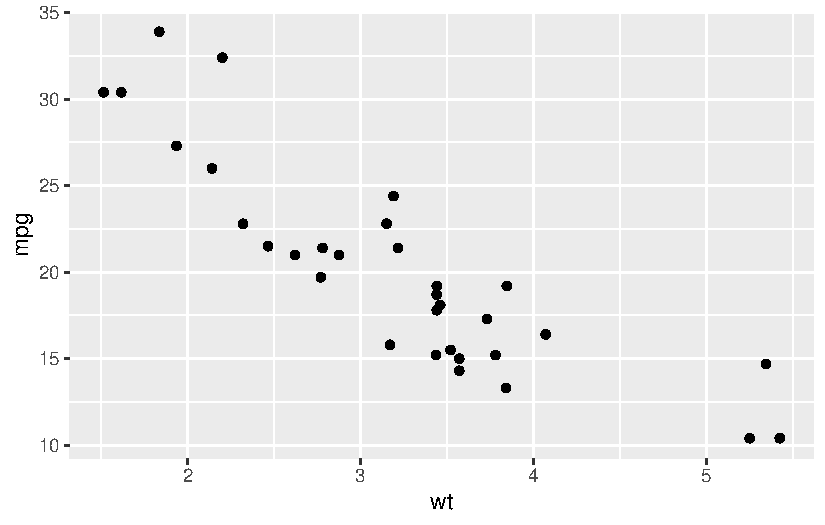
\includegraphics[keepaspectratio]{04-resultados_files/figure-pdf/grafico-ejemplo-1.pdf}}

}

\end{figure}%

\section{Modelos}\label{modelos}

Presentacion de los resultados de los modelos propuestos, con
interpretacion y conclusiones.

\begin{longtable}[]{@{}
  >{\raggedright\arraybackslash}p{(\linewidth - 12\tabcolsep) * \real{0.2738}}
  >{\centering\arraybackslash}p{(\linewidth - 12\tabcolsep) * \real{0.0952}}
  >{\centering\arraybackslash}p{(\linewidth - 12\tabcolsep) * \real{0.1310}}
  >{\centering\arraybackslash}p{(\linewidth - 12\tabcolsep) * \real{0.1071}}
  >{\centering\arraybackslash}p{(\linewidth - 12\tabcolsep) * \real{0.1071}}
  >{\centering\arraybackslash}p{(\linewidth - 12\tabcolsep) * \real{0.0714}}
  >{\centering\arraybackslash}p{(\linewidth - 12\tabcolsep) * \real{0.2143}}@{}}
\caption{Resumen comparativo de modelos}\tabularnewline
\toprule\noalign{}
\begin{minipage}[b]{\linewidth}\raggedright
Predictor
\end{minipage} & \begin{minipage}[b]{\linewidth}\centering
Coef.
\end{minipage} & \begin{minipage}[b]{\linewidth}\centering
Std. Err.
\end{minipage} & \begin{minipage}[b]{\linewidth}\centering
t-valor
\end{minipage} & \begin{minipage}[b]{\linewidth}\centering
p-valor
\end{minipage} & \begin{minipage}[b]{\linewidth}\centering
Sig.
\end{minipage} & \begin{minipage}[b]{\linewidth}\centering
IC 95 \%
\end{minipage} \\
\midrule\noalign{}
\endfirsthead
\toprule\noalign{}
\begin{minipage}[b]{\linewidth}\raggedright
Predictor
\end{minipage} & \begin{minipage}[b]{\linewidth}\centering
Coef.
\end{minipage} & \begin{minipage}[b]{\linewidth}\centering
Std. Err.
\end{minipage} & \begin{minipage}[b]{\linewidth}\centering
t-valor
\end{minipage} & \begin{minipage}[b]{\linewidth}\centering
p-valor
\end{minipage} & \begin{minipage}[b]{\linewidth}\centering
Sig.
\end{minipage} & \begin{minipage}[b]{\linewidth}\centering
IC 95 \%
\end{minipage} \\
\midrule\noalign{}
\endhead
\bottomrule\noalign{}
\endlastfoot
Constante & 37.227 & 1.599 & 23.28 & \textless0.001 & *** & {[}33.957,
40.497{]} \\
Capital social barrial & -3.878 & 0.633 & -6.13 & \textless0.001 & *** &
{[}-5.172, -2.584{]} \\
Precariedad laboral & -0.032 & 0.009 & -3.52 & 0.001 & ** & {[}-0.050,
-0.013{]} \\
N & 32 & & & & & \\
R\^{}2 & 0.827 & & & & & \\
R\^{}2 ajustado & 0.815 & & & & & \\
\end{longtable}

\bookmarksetup{startatroot}

\chapter{Discusión}\label{discusiuxf3n}

Interpreta resultados, limitaciones y aportes.

\bookmarksetup{startatroot}

\chapter{Conclusiones}\label{conclusiones}

Síntesis y proyecciones futuras.

\bookmarksetup{startatroot}

\chapter{Referencias}\label{referencias}

\phantomsection\label{refs}
\begin{CSLReferences}{1}{0}
\bibitem[\citeproctext]{ref-bourdieu2012}
Bourdieu, P. (2012). \emph{La distinci{ó}n: Criterio y bases sociales
del gusto}. Taurus.

\bibitem[\citeproctext]{ref-desmond2019poverty}
Desmond, M., \& Wilmers, N. (2019). The Racialized Geography of Housing.
\emph{American Journal of Sociology}.

\bibitem[\citeproctext]{ref-xie2017bookdown}
Xie, Y. (2017). \emph{bookdown: Authoring Books and Technical Documents
with R Markdown}. Chapman; Hall/CRC.

\end{CSLReferences}

\cleardoublepage
\phantomsection
\addcontentsline{toc}{part}{Apéndices}
\appendix

\chapter{Instrumentos de
levantamiento}\label{instrumentos-de-levantamiento}

Incluye cuestionarios, guias de entrevista, etc.

\chapter{Tablas adicionales}\label{tablas-adicionales}

Tablas extendidas, tests de robustez, etc.


\backmatter

% --- Cuerpo del libro (capítulos) en arábigos ---
\mainmatter
\pagestyle{scrheadings}

% --- (Opcional) Estilo del índice general ---
% \addtocontents{toc}{\protect\thispagestyle{plain}}


\end{document}
